\documentclass{article}
\usepackage[utf8]{inputenc}
\usepackage{amsmath}
\usepackage{amsfonts}
\usepackage{amssymb}
\usepackage{mathtools}
\usepackage{graphicx}
\usepackage{booktabs}
\usepackage{subcaption}
\usepackage[ruled,linesnumbered,commentsnumbered]{algorithm2e}
\DeclarePairedDelimiter\abs{\lvert}{\rvert}%
\DeclarePairedDelimiter\norm{\lVert}{\rVert}%
% Swap the definition of \abs* and \norm*, so that \abs
% and \norm resizes the size of the brackets, and the 
% starred version does not.
\makeatletter
\let\oldabs\abs
\def\abs{\@ifstar{\oldabs}{\oldabs*}}
%
\let\oldnorm\norm
\def\norm{\@ifstar{\oldnorm}{\oldnorm*}}
\makeatother

\title{A novel adaptive learning rate scheduler for deep neural networks}
\author{Rahul Yedida and Snehanshu Saha}
\date{}
\begin{document}
\maketitle

\begin{abstract}
    Optimizing deep neural networks is largely thought to be an empirical process, requiring manual tuning of several parameters, such as learning rate, weight decay, and dropout rate. Arguably, the learning rate is the most important of these to tune, and this has gained more attention in recent works. In this paper, we propose a novel method to compute the learning rate for training deep neural networks. We derive a theoretical framework to compute learning rates dynamically, and then show experimental results on standard datasets and architectures to demonstrate the efficacy of our approach.
\end{abstract}

\section{Introduction}
Deep learning \cite{goodfellow2016deep} is becoming more omnipresent for several tasks, including image recognition \cite{simonyan2014very, szegedy2015going}, face recognition \cite{taigman2014deepface}, and object detection \cite{girshick2014rich}.  At the same time, the trend is towards deeper neural networks \cite{ioffe2015batch,he2015delving}.

Deep convolutional neural networks \cite{krizhevsky2012imagenet,lecun1989backpropagation} are a variant that introduce convolutional and pooling layers, and have seen incredible success in image classification \cite{sermanet2013overfeat,zeiler2014visualizing}, even surpassing human-level performance \cite{he2015delving}. Very deep convolutional neural networks have even crossed 1000 layers \cite{he2016identity}.

Despite their popularity, training neural networks is made difficult by several problems. These include vanishing and exploding gradients \cite{glorot2010understanding,bengio1994learning} and overfitting. Various advances including different activation functions \cite{klambauer2017self,nair2010rectified}, batch normalization \cite{ioffe2015batch}, novel initialization schemes \cite{he2015delving}, and dropout \cite{srivastava2014dropout} offer solutions to these problems. 

However, a more fundamental problem is that of finding optimal values for various hyperparameters, of which the learning rate is arguably the most important. It is well-known that learning rates that are too small are slow to converge, while learning rates that are too large cause divergence \cite{bengio2012neural}. Recent works agree that rather than a fixed learning rate value, a non-monotonic learning rate scheduling system offers faster convergence \cite{seong2018towards,smith2017cyclical}. It has also been argued that the traditional wisdom that large learning rates should not be used may be flawed, and can lead to ``super-convergence" and have regularizing effects \cite{smith2017super}. Our experimental results agree with this statement; however, rather than use cyclical learning rates based on intuition, we propose a novel method to compute an adaptive learning rate backed by theoretical foundations. 

To the best of our knowledge, this is the first work to suggest an adaptive learning rate scheduler with a theoretical background and show experimental verification of its claim on standard datasets and network architectures. Thus, our contributions are two-fold. First, we propose a novel theoretical framework for computing an optimal learning rate in stochastic gradient descent in deep neural networks, based on the Lipschitz constant of the loss function. We show that for certain choices of activation functions, only the activations in the last two layers are required to compute the learning rate. Second, we compute the ideal learning rate for several commonly used loss functions, and use these formulas to experimentally demonstrate the efficacy of our approach.

Our approach exploits functional properties of the loss function, and only makes two minimal assumptions on the loss function: it must be Lipschitz continuous\cite{saha} and (at least) once differentiable. Commonly used loss functions satisfy both these properties.

The rest of the paper is organized as follows. Section 3 introduces our novel theoretical framework. Sections 4 to 6 derive the learning rates for some common loss functions. Section 7 then shows experimental results demonstrating the benefits of our approach. Finally, Section 8 concludes and discusses possible future work.

\section{Related Work}
Several enhancements to the original gradient descent algorithm have been proposed. These include adding a ``momentum" term to the update rule \cite{sutskever2013importance}, and ``adaptive gradient" methods such as RMSProp\cite{tieleman2012lecture}, and Adam\cite{kingma2014adam}, which combines RMSProp and AdaGrad\cite{duchi2011adaptive}. These methods have seen widespread use in deep neural networks\cite{radford2015unsupervised,xu2015show,bahar2017empirical}.

Recently, there has been a lot of work on finding novel ways to adaptively change the learning rate. These have both theoretical \cite{seong2018towards} and intuitive, empirical \cite{smith2017super, smith2017cyclical} backing. These works rely on non-monotonic scheduling of the learning rate. \cite{smith2017cyclical} argues for cyclical learning rates. Our proposed method also yields a non-monotonic learning rate, but does not follow any predefined shape.

Our work is also motivated by recent works that theoretically show that stochastic gradient descent is sufficient to optimize over-parameterized neural networks, making minimal assumptions \cite{zou2018stochastic,du2018gradient}. Our aim is to mathematically identify an optimal learning rate, rejecting the notion that only small learning rates must be used, and then experimentally show the validity of our claims.

\section{Theoretical framework}
For a neural network that uses the sigmoid, ReLU, or softmax activations, it is easily shown that the gradients get smaller towards the earlier layers in backpropagation. Because of this, the gradients at the last layer are the maximum among all the gradients computed during backpropagation. If $w^{[l]}_{ij}$ is the weight from node $i$ to node $j$ at layer $l$, and if $L$ is the number of layers, then
\begin{equation}
	\max\limits_{h, k} \frac{\partial E}{\partial w^{[L]}_{hk}} \geq \frac{\partial E}{\partial w^{[l]}_{ij}} \forall\  l, i, j \label{eq:int:1}
\end{equation}

Essentially, \eqref{eq:int:1} says that the maximum gradient of the error with respect to the weights in the last layer is greater than the gradient of the error with respect to any weight in the network. This obviously extends to the bias as well. In other words, finding the maximum gradient at the last layer gives us a supremum of the Lipschitz constants of the error, where the gradient is taken with respect to the weights at any layer.

We now analytically arrive at a theoretical supremum value for different types of problems. The inverse of these values can be used as a learning rate in gradient descent. In any layer, we have the computations
\begin{align}
	z^{[l]} &= W^{[l]T}a^{[l-1]} + b^{[l]} \label{eq:int:2} \\
	a^{[l]} &= g(z^{[l]}) \label{eq:int:3} \\
	a^{[0]} &= X \label{eq:int:4}
\end{align}
Thus, the gradient with respect to any weight in the last layer is computed via the chain rule as follows.
\begin{align}
	\frac{\partial E}{\partial w^{[L]}_{ij}} &= \frac{\partial E}{\partial a^{[L]}_j}\cdot \frac{\partial a^{[L]}_j}{\partial z^{[L]}_j}\cdot \frac{\partial z^{[L]}_j}{\partial w^{[L]}_{ij}} \nonumber  \\
	&= \frac{\partial E}{\partial a^{[L]}_j}\cdot \frac{\partial a^{[L]}_j}{\partial z^{[L]}_j}\cdot a^{[L-1]}_j \label{eq:int:5}
\end{align}
This gives us
\begin{equation}
	\max\limits_{i,j} \abs{\frac{\partial E}{\partial w^{[L]}_{ij}}} = \max\limits_j \abs{ \frac{\partial E}{\partial a^{[L]}_j} }\cdot \max\limits_j \abs{ \frac{\partial a^{[L]}_j}{\partial z^{[L]}_j} }\cdot \max\limits_j \abs{ a^{[L-1]}_j } \label{eq:int:6}
\end{equation}
The third part cannot be analytically computed; we denote it as $K_z$. We now look at various types of problems and compute these components.

\section{Regression}
For regression, we use the least-squares cost function. Further, we assume that there is only one output node. That is,
\begin{equation}
	E(\textbf{a}^{[L]}) = \frac{1}{2m} \left( \textbf{a}^{[L]} - \textbf{y} \right)^2 \label{eq:reg:1}
\end{equation}
where the vectors contain the values for each training example. Then we have,
\begin{align*}
	E(\textbf{b}^{[L]}) - E(\textbf{a}^{[L]}) &= \frac{1}{2m} \left( \left( \textbf{b}^{[L]} - \textbf{y} \right)^2 - \left( \textbf{a}^{[L]} - \textbf{y} \right)^2 \right) \\
	&= \frac{1}{2m} \left( \textbf{b}^{[L]} + \textbf{a}^{[L]} - 2\textbf{y} \right) \left( \textbf{b}^{[L]} - \textbf{a}^{[L]} \right)
\end{align*}
This gives us,
\begin{align}
	\frac{\lVert E(\textbf{b}^{[L]}) - E(\textbf{a}^{[L]}) \rVert}{\lVert \textbf{b}^{[L]} - \textbf{a}^{[L]} \rVert} &= \frac{1}{2m} \lVert \textbf{b}^{[L]} + \textbf{a}^{[L]} - 2\textbf{y} \rVert \nonumber \\
	& \leq \frac{1}{m} \left( K_a - \lVert y \rVert \right) \label{eq:reg:2}
\end{align}
where $K_a$ is the upper bound of $\lVert \textbf{a} \rVert$ and $\lVert \textbf{b} \rVert$. A reasonable choice of norm is the 2-norm.

Looking back at \eqref{eq:int:6}, the second term on the right side of the equation is the derivative of the activation with respect to its parameter. Notice that if the activation is sigmoid or softmax, then it is necessarily less than 1; if it is ReLu, it is either 0 or 1. Therefore, to find the maximum, we assume that the network is comprised solely of ReLu activations, and the maximum of this is 1.

From \eqref{eq:int:6}, we have
\begin{equation}
	\max\limits_{i,j} \abs{ \frac{\partial E}{\partial w^{[L]}_{ij}} } = \frac{1}{m} \left( K_a - \lVert y \rVert \right) K_z
\end{equation}
The inverse of this, therefore, can be set as the learning rate for gradient descent.

\section{Binary classification}
For binary classification, we use the binary cross-entropy loss function. Assuming only one output node,
\begin{equation}
    E(\textbf{z}^{[L]}) = -\frac{1}{m} \left( \textbf{y} \log g(\textbf{z}^{[L]}) + (1-\textbf{y}) \log (1 - g(\textbf{z}^{[L]})) \right) \label{eq:bin:1}
\end{equation}
where $g(z)$ is the sigmoid function. We use a slightly different version of \eqref{eq:int:6} here:
\begin{equation}
    \max\limits_{i,j} \abs{ \frac{\partial E}{\partial w^{[L]}_{ij}} } = \max\limits_j \abs{ \frac{\partial E}{\partial z^{[L]}_j} }\cdot K_z \label{eq:bin:2}
\end{equation}
Then, we have
\begin{align}
    \frac{\partial E}{\partial \textbf{z}^{[L]}} &= -\frac{1}{m} \left( \frac{\textbf{y}}{g(\textbf{z}^{[L]})}g(\textbf{z}^{[L]})(1-g(\textbf{z}^{[L]})) - \frac{1-\textbf{y}}{1-g(\textbf{z}^{[L]})}g(\textbf{z}^{[L]})(1-g(\textbf{z}^{[L]})) \right) \nonumber \\
    &= -\frac{1}{m}\left( \textbf{y}(1-g(\textbf{z}^{[L]})) - (1-\textbf{y})g(\textbf{z}^{[L]}) \right) \nonumber \\
    &= -\frac{1}{m}\left( \textbf{y} - \textbf{y}g(\textbf{z}^{[L]}) - g(\textbf{z}^{[L]}) + \textbf{y}g(\textbf{z}^{[L]}) \right) \nonumber \\
    &= -\frac{1}{m}\left( \textbf{y} - g(\textbf{z}^{[L]}) \right) \label{eq:bin:3}
\end{align}
It is easy to show, using the second derivative, that this attains a maxima at $\textbf{z}^{[L]}=0$:
\begin{equation}
    \frac{\partial^2 E}{\partial \textbf{w}^{[L]2}_{ij}} = \frac{1}{m}g(\textbf{z}^{[L]})(1 - g(\textbf{z}^{[L]})) a^{[L-1]}_j \label{eq:bin:4}
\end{equation}
Setting \eqref{eq:bin:4} to 0 yields $a^{[L-1]}_j = 0\ \forall j$, and thus $z^{[L]} = W^{[L]}_{ij}a^{[L-1]}_j = 0$. This implies $g(\textbf{z}^{[L]}) = \frac{1}{2}$. Now whether $\textbf{y}$ is 0 or 1, substituting this back in \eqref{eq:bin:3}, we get
\begin{equation}
    \max_j \abs{ \frac{\partial E}{\partial z^{[L]}_j} } = \frac{1}{2m} \label{eq:bin:5}
\end{equation}
Using \eqref{eq:bin:5} in \eqref{eq:bin:2},
\begin{equation}
    \max\limits_{i,j} \abs{ \frac{\partial E}{\partial w^{[L]}_{ij}} } = \frac{K_z}{2m} \label{eq:bin:6}
\end{equation}

\section{General cross-entropy loss function}
While conventionally, multi-class classification is done using one-hot encoded outputs, that is not convenient to work with mathematically. An identical form of this is to assume the output follows a Multinomial distribution, and then updating the loss function accordingly. This is because the effect of the typical loss function used is to only consider the ``hot" vector; we achieve the same effect using the Iverson notation, which is equivalent to the Kronecker delta. With this framework, the loss function is
\begin{equation}
     E(\textbf{a}^{[L]}) = -\frac{1}{m} \sum\limits_{j=1}^k [\textbf{y}=j] \log \textbf{a}^{[L]} \label{eq:mul:1}
\end{equation}
Then the first part of \eqref{eq:int:6} is trivial to compute:
\begin{equation}
    \frac{\partial E}{\partial \textbf{a}^{[L]}} = -\frac{1}{m} \sum\limits_{j=1}^m \frac{[\textbf{y}=j]}{\textbf{a}^{[L]}} \label{eq:mul:2}
\end{equation}
The second part is computed as follows.
\begin{align} 
    \frac{\partial a^{[L]}_j}{\partial z^{[L]}_p} &= \frac{\partial}{\partial z^{[L]}_p} \left( \frac{e^{z^{[L]}_j}}{\sum_{l=1}^k e^{z^{[L]}_l}} \right) \nonumber \\ 
    &= \frac{[p=j] e^{z^{[L]}_j}\sum_{l=1}^k e^{z^{[L]}_l } - e^{z^{[L]}_j } \cdot e^{z^{[L]}_p} }{\left( \sum_{l=1}^k e^{z^{[L]}_l } \right)^2} \nonumber \\ 
    &= \frac{[p=j] e^{z^{[L]}_j }}{\sum_{l=1}^k e^{z^{[L]}_l }} - \frac{e^{z^{[L]}_j }}{\sum_{l=1}^k e^{z^{[L]}_l }} \cdot \frac{e^{z^{[L]}_p }}{\sum_{l=1}^k e^{z^{[L]}_l }} \nonumber \\ 
    &= \left([p=j] a^{[L]}_j - a^{[L]}_j a^{[L]}_p \right) \nonumber \\ 
    &= a^{[L]}_j([p=j]-a^{[L]}_p) \label{eq:mul:3}
\end{align}
Combining \eqref{eq:mul:2} and \eqref{eq:mul:3} in \eqref{eq:int:5} gives
\begin{equation}
    \frac{\partial E}{\partial W^{[L]}_p} = \frac{1}{m} \left( a^{[L]}_p - [\textbf{y}=p] \right)K_z \label{eq:mul:4}
\end{equation}
It is easy to show that the limiting case of this is when all softmax values are equal and each $y^{(i)}=p$; using this and $a^{[L]}_p = \frac{1}{k}$ in \eqref{eq:mul:4} and combining with \eqref{eq:int:6} gives us our desired result:
\begin{equation}
    \max\limits_j \abs{ \frac{\partial E}{\partial W^{[L]}_j} } = \frac{k-1}{km}K_z \label{eq:mul:5}
\end{equation}

\section{A note on regularization} \label{regularization}
It should be noted that this framework is extensible to the case where the loss function includes a regularization term. 

In particular, if an $L_2$ regularization term, $\frac{\lambda}{2}\left\Vert \textbf{w} \right\Vert_2^2$ is added, it is trivial to show that the Lipschitz constant increases by $\lambda K$, where $K$ is the upper bound for $\left\Vert \textbf{w} \right\Vert$. More generally, if a Tikhonov regularization term, $\left\Vert \boldsymbol\Gamma \textbf{w} \right\Vert_2^2$ term is added, then the increase in the Lipschitz constant can be computed as below.

\[
    \begin{aligned}
        L(\textbf{w}_1) - L(\textbf{w}_2) &= (\boldsymbol\Gamma \textbf{w}_1)^T (\boldsymbol\Gamma \textbf{w}_1) - (\boldsymbol\Gamma \textbf{w}_2)^T (\boldsymbol\Gamma \textbf{w}_2) \\
        &= \textbf{w}_1^T \boldsymbol\Gamma^2 \textbf{w}_1 - \textbf{w}_2^T \boldsymbol\Gamma^2 \textbf{w}_2 \\
        &= 2\textbf{w}_2^T \boldsymbol\Gamma^2 (\textbf{w}_1 - \textbf{w}_2) + (\textbf{w}_1-\textbf{w}_2)^T \Gamma^2 (\textbf{w}_1-\textbf{w}_2) \\
        \frac{\left\Vert L(\textbf{w}_1) - L(\textbf{w}_2) \right\Vert}{\left\Vert \textbf{w}_1-\textbf{w}_2 \right\Vert} & \leq 2 \left\Vert \textbf{w}_2 \right\Vert \left\Vert \boldsymbol\Gamma^2 \right\Vert + \left\Vert \textbf{w}_1-\textbf{w}_2 \right\Vert \left\Vert \boldsymbol\Gamma^2 \right\Vert 
    \end{aligned}
\]

If $\textbf{w}_1, \textbf{w}_2$ are bounded by $K$, 

\[
    \boxed{
        L = 2K \left\Vert \boldsymbol\Gamma^2 \right\Vert
    }
\]

This additional term may be added to the Lipschitz constants derived above when gradient descent is performed on a loss function including a Tikhonov regularization term. Clearly, for an $L_2$-regularizer, since $\boldsymbol\Gamma = \frac{\lambda}{2}\textbf{I}$, $L = \lambda K$.

\section{Going Beyond SGD}
The framework presented thus far easily extends to algorithms that extend SGD, such as RMSprop, momentum, and Adam. In this section, we show algorithms for some major optimization algorithms popularly used. Further, we show experients for Adam, since it combines the other methods.

RMSprop, gradient descent with momentum, and Adam are based on exponentially weighted averages of the gradients. The trick then is to compute the Lipschitz constant as an exponentially weighted average of the norms of the gradients. This makes sense, since it provides a supremum of the ``velocity" or ``accumulator" terms in momentum and RMSprop respectively.

\subsection{Gradient Descent with Momentum}
SGD with momentum uses an exponentially weighted average of the gradient as a velocity term. The gradient is replaced by the velocity in the weight update rule.

\begin{algorithm}[H]
    \SetAlgoLined
    $K \gets 0$; $V_{\nabla L} \gets 0$\;
    \For{each iteration}{
        Compute $\nabla_W L$ for all layers\;
        $V_{\nabla L} \gets \beta V_{\nabla L} + (1-\beta) \nabla_W L$\;
        \tcp{Compute the exponentially weighted average of LC}
        $K \gets \beta K + (1-\beta) \max \norm{\nabla_W L}$ \label{algo:mom:lc}\;
        \tcp{Weight update}
        $W \gets W - \frac{1}{K}V_{\nabla L}$ \label{algo:mom:update}\;
    }
    \caption{Adaptive momentum}
    \label{algo:mom}
\end{algorithm}

Algorithm \ref{algo:mom} shows the \textit{adaptive} version of gradient descent with momentum. The only changes are on lines \ref{algo:mom:lc} and \ref{algo:mom:update}. The exponentially weighted average of the Lipschitz constant ensures that the learning rate for that iteration is optimal. The weight update is changed to reflect our new learning rate. We use the symbol $W$ to consistently refer to the weights as well as the biases; while ``parameters" may be a more apt term, we use $W$ to stay consistent with literature.

Notice that only line \ref{algo:mom:lc} is our job; deep learning frameworks will typically take care of the rest; we simply need to compute $K$ and use a learning rate scheduler that uses the inverse of this value.

\subsection{RMSprop}
RMSprop uses an exponentially weighted average of the square of the gradients. The square is performed element-wise, and thus preserves dimensions. The update rule in RMSprop replaces the gradient with the ratio of the current gradient and the exponentially moving average. A small value $\epsilon$ is added to the denominator for numerical stability.

Algorithm \ref{algo:rms} shows the modified version of RMSprop. We simply maintain an exponentially weighted average of the Lipschitz constant as before; the learning rate is also replaced by the inverse of the update term, with the exponentially weighted average of the square of the gradient replaced with our computed exponentially weighted average.

\begin{algorithm}[H]
    \SetAlgoLined
    $K \gets 0$; $S_{\nabla L} \gets 0$\;
    \For{each iteration}{
        Compute $\nabla_W L$ on mini-batch\;
        $S_{\nabla L} \gets \beta S_{\nabla L} + (1-\beta) (\nabla_W L)^2$\;
        \tcp{Compute the exponentially weighted average of LC}
        $K \gets \beta K + (1-\beta) \max \norm{(\nabla_W L)^2}$ \label{algo:rms:lc}\;
        \tcp{Weight update}
        $W \gets W - \frac{\sqrt{K} + \epsilon}{\max \norm{\nabla_{W} L}}\cdot \frac{\nabla_{W} L}{\sqrt{S_{\nabla L\textit{}}} + \epsilon}$ \label{algo:rms:update}\;
    }
    \caption{Adaptive RMSprop}
    \label{algo:rms}
\end{algorithm}

\subsection{Adam}
Adam combines the above two algorithms. We thus need to maintain two exponentially weighted average terms. The algorithm, shown in Algorithm \ref{algo:adam}, is quite straightforward.

\begin{algorithm}[H]
    \SetAlgoLined
    $K_1 \gets 0$; $K_2 \gets 0$; $S_{\nabla L} \gets 0$; $V_{\nabla L} = 0$\;
    \For{each iteration}{
        Compute $\nabla_W L$ on mini-batch\;
        $V_{\nabla L} \gets \beta_1 V_{\nabla L} + (1-\beta_1) \nabla_W L$\;
        $S_{\nabla L} \gets \beta_2 S_{\nabla L} + (1-\beta_2) (\nabla_W L)^2$\;
        \tcp{Compute the exponentially weighted averages of LC}
        $K_1 \gets \beta_1 K_1 + (1-\beta_1) \max \norm{\nabla_W L}$ \;
        $K_2 \gets \beta_2 K_2 + (1-\beta_2) \max \norm{(\nabla_W L)^2}$ \;
        \tcp{Weight update}
        $W \gets W - \frac{\sqrt{K_2} + \epsilon}{K_1}\cdot \frac{V_{\nabla L}}{\sqrt{S_{\nabla L\textit{}}} + \epsilon}$ \label{algo:adam:update}\;
    }
    \caption{Auto-Adam}
    \label{algo:adam}
\end{algorithm}

In our experiments, we use the defaults of $\beta_1 = 0.9, \beta_2 = 0.999$.

\subsection{A note on bias correction}
While not commonly used, some implementations of the above algorithms perform bias correction as well. This involves computing the exponentially weighted average, and then dividing by $1 - \beta^t$, where $t$ is the epoch number. In this case, the above algorithms may be adjusted by also dividing the Lipschitz constants by the same constant.

\section{Experiments}
Below we show the results and details of our experiments on some publicly available datasets. While our results are not state of the art, our focus was to empirically show that SGD can be run with higher learning rates than typically understood. All our experiments were run on a Tesla P100 GPU, and the models were optimized using a stochastic gradient descent optimizer with no momentum or weight decay unless specified. On CIFAR, we only use flipping and translation augmentation schemes as in \cite{he2016deep}. In all experiments the raw image values were divided by 255.

\subsection{MNIST}
\begin{table}
    \centering
    \caption{CNN used for MNIST}
    \begin{tabular}{ccc}
        \toprule \\
        Layer & Filters & Padding \\
        \midrule \\
        3 x 3 Conv & 32 & Valid  \\
        3 x 3 Conv & 32 & Valid  \\
        2 x 2 MaxPool & -- & -- \\
        Dropout (0.2) & -- & -- \\
        3 x 3 Conv & 64 & Same \\
        3 x 3 Conv & 64 & Same \\
        2 x 2 MaxPool & -- & -- \\
        Dropout (0.25) & -- & -- \\
        3 x 3 Conv & 128 & Same \\
        Dropout (0.25) & -- & -- \\
        Flatten & -- & -- \\
        Dense (128) & -- & -- \\
        BatchNorm & -- & -- \\
        Dropout (0.25) & -- & -- \\
        Dense (10) & -- & -- \\
        \bottomrule \\
    \end{tabular}
    \label{tab:mnist:1}
\end{table}

On MNIST, the architecture we used is shown in Table \ref{tab:mnist:1}. All activations except the last layer are ReLU; the last layer uses softmax activations. The model has 730K parameters. We trained the model on a Tesla K80 GPU.

Our preprocessing involved random shifts (up to 10\%), zoom (to 10\%), and rotations (to $15^\circ$). We used a batch size of 256, and ran the model for 20 epochs. Each epoch took around 18 seconds. The experiment on MNIST used only an adaptive learning rate, where the Lipschitz constant, and therefore, the learning rate was recomputed every epoch. Note that this works even though the penultimate layer is a Dropout layer. No regularization was used during training. With these settings, we achieved a training accuracy of 98.57\% and validation accuracy 99.5\%. 

\begin{figure}
    \centering
    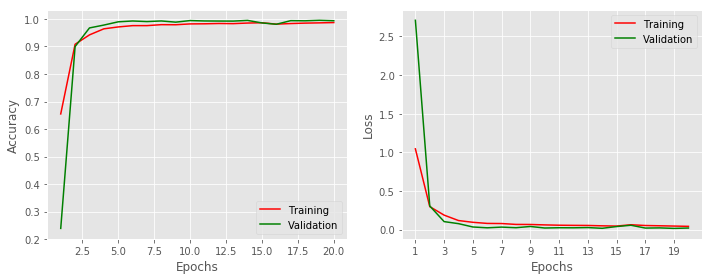
\includegraphics[scale=0.4]{mnist-plot.png}
    \caption{Plot of accuracy score and loss over epochs on MNIST}
    \label{fig:mnist:1}
\end{figure}

Figure \ref{fig:mnist:1} shows the plot of accuracy scores and loss over the training and validation sets over epochs.

\begin{figure}
    \centering
    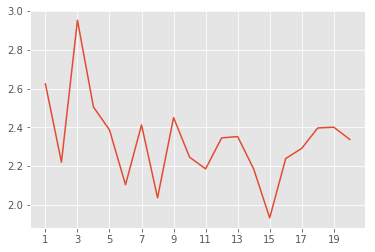
\includegraphics[scale=0.4]{mnist-lr.png}
    \caption{Adaptive learning rate over time on MNIST}
    \label{fig:mnist:2}
\end{figure}

Finally, Figure \ref{fig:mnist:2} shows the computed learning rate over epochs. Note that unlike the computed adaptive learning rates for CIFAR-10 (Figure \ref{fig:cifar10:3}) and CIFAR-100 (Figure \ref{fig:cifar100:1}), the learning rate for MNIST starts at a much higher value. While the learning rate here seems much more random, it must be noted that this was run for only 20 epochs, and hence any variation is exaggerated in comparison to the other models, run for 300 epochs.

\subsection{CIFAR-10}
For the CIFAR-10 experiments, we used a ResNet20 v1\cite{he2016deep}. A residual network is a deep neural network that is made of ``residual blocks". A residual block is a special case of a highway networks \cite{srivastava2015highway} that do not contain any gates in their skip connections. ResNet v2 also uses ``bottleneck" blocks. A bottleneck residual unit consist of a 1x1 layer for reducing dimension, a 3x3 layer, and a 1x1 layer for restoring dimension \cite{he2016identity}. More details can be found in the original ResNet papers \cite{he2016deep,he2016identity}.

We ran two sets of experiments on CIFAR-10. First, we empirically computed $K_z$ by running one epoch and finding the activations of the penultimate layer. We ran our model for 300 epochs using the same fixed learning rate. Each epoch took 24 seconds on average. We used a batch size of 128, and a weight decay of $10^{-3}$. Our computed values of $K_z$, $\max \norm{w}$, and learning rate were 206.695, 43.257, and 0.668 respectively. It should be noted that while computing the Lipschitz constant, $m$ in the denominator must be set to the batch size, not the total number of training examples. In our case, we set it to 128. 

\begin{figure}
    \centering
    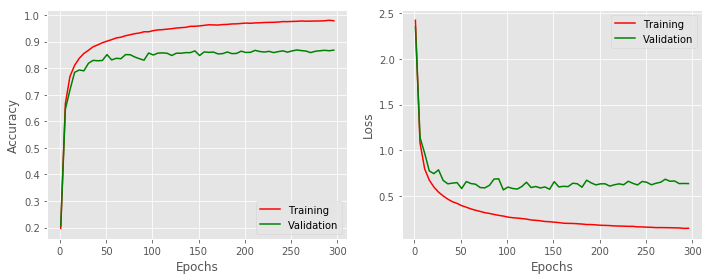
\includegraphics[scale=0.4]{plot-cifar10.png}
    \caption{Plot of accuracy score and loss over epochs on CIFAR-10}
    \label{fig:cifar10:1}
\end{figure}

Figure \ref{fig:cifar10:1} shows the plots of accuracy score and loss over time. As noted in \cite{smith2018disciplined}, a horizontal validation loss indicates little overfitting. We achieved a training accuracy of 97.61\% and a  validation accuracy of 87.02\% with these settings.

\begin{figure}
    \centering
    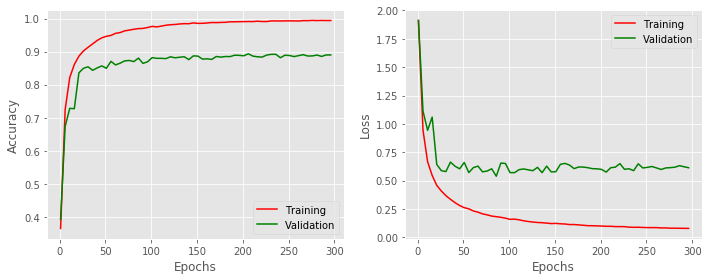
\includegraphics[scale=0.4]{adaptive-plots-cifar10.png}
    \caption{Plot of accuracy score and loss over epochs on CIFAR-10 with adaptive learning rate}
    \label{fig:cifar10:2}
\end{figure}

Second, we used the same hyperparameters as above, but recomputed $K_z$, $\max \norm{w}$, and the learning rate every epoch. This cost us around 3 extra seconds per epoch on average. Figure \ref{fig:cifar10:2} shows the plots of accuracy scores and loss over epochs for this setting. We obtained a training accuracy of 99.47\%, validation accuracy of 89.37\%, and test accuracy of 89.03\%. Clearly, this method is superior to a fixed learning rate policy. 

\begin{figure}
    \centering
    \begin{subfigure}[b]{0.4\textwidth}
        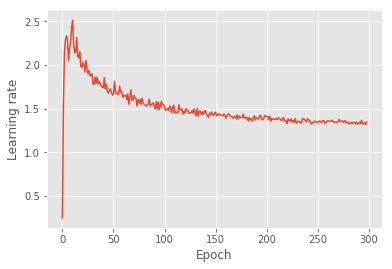
\includegraphics[width=\linewidth]{cifar10-lr-full.png}
        \caption{Learning rate over epochs}
        \label{fig:cifar10:3a}
    \end{subfigure}
    \begin{subfigure}[b]{0.4\textwidth}
        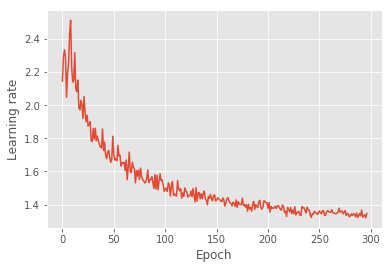
\includegraphics[width=\linewidth]{adaptive-lr.png}
        \caption{Learning rate from epoch 2}
        \label{fig:cifar10:3b}
    \end{subfigure}
    \caption{Adaptive learning rate over time on CIFAR-10}
    \label{fig:cifar10:3}
\end{figure}

Figure \ref{fig:cifar10:3} shows the learning rate over time. The adaptive scheme automatically chooses a decreasing learning rate, as suggested by literature on the subject. On the first epoch, however, the model chooses a very small learning rate of $8 \times 10^{-3}$, owing to the random initialization. 

Note that while it does follow the conventional wisdom of choosing a higher learning rate initially to explore the weight space faster and then slowing down as it approaches the global minimum, it ends up choosing a significantly larger learning rate than traditionally used. Clearly, there is no need to decay learning rate by a multiplicative factor. Our model with adaptive learning rate outperforms our model with a fixed learning rate in only 65 epochs. Further, the generalization error is lower with the adaptive learning rate scheme using the same weight decay value. This seems to confirm the notion in \cite{smith2017super} that large learning rates have a regularization effect.

\subsection{CIFAR-100}
For the CIFAR-100 experiments, we used a ResNet164 v2 \cite{he2016identity}. Our experiments on CIFAR-100 only used an adaptive learning rate scheme.

We largely used the same parameters as before. Data augmentation involved only flipping and translation. We ran our model for 300 epochs, with a batch size of 128. Each epoch took 139 seconds on average on a P100 GPU. As in \cite{he2016identity}, we used a weight decay of $10^{-4}$. We achieved a training accuracy of 99.68\%, validation accuracy of 75.99\%, and test accuracy of 73.26\% with these settings.

\begin{figure}
    \centering
    \begin{subfigure}[b]{0.4\textwidth}
        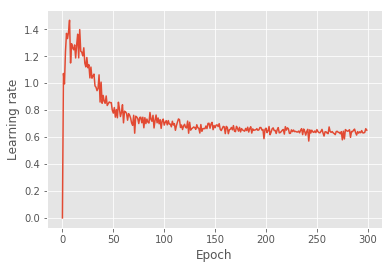
\includegraphics[width=\linewidth]{cifar100-lr-full.png}
        \caption{Learning rate over epochs}
        \label{fig:cifar100:1a}
    \end{subfigure}
    \begin{subfigure}[b]{0.4\textwidth}
        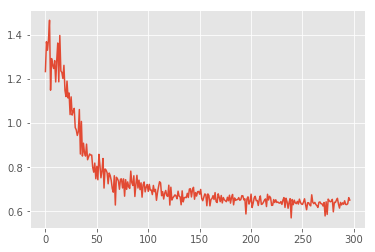
\includegraphics[width=\linewidth]{cifar100-lr-3.png}
        \caption{Learning rate from epoch 3}
        \label{fig:cifar100:1b}
    \end{subfigure}
    \caption{Adaptive learning rate over time on CIFAR-100}
    \label{fig:cifar100:1}
\end{figure}

Figure \ref{fig:cifar100:1} shows the learning rate over epochs. As with CIFAR-10, the first two epochs start off with a very small ($10^{-8}$) learning rate, but the model quickly adjusts to changing weights.

\begin{figure}
    \centering
    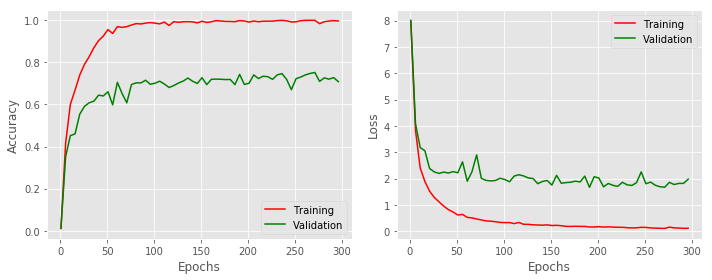
\includegraphics[scale=0.4]{plot-rn162.png}
    \caption{Accuracy scores and loss values over epochs on CIFAR-100}
    \label{fig:cifar100:2}
\end{figure}

Figure \ref{fig:cifar100:2} shows the accuracy scores and loss values on the training and validation sets over epochs.

\section{Conclusion and Future Work}
In this paper, we derived a theoretical framework for computing an adaptive learning rate; on deriving the formulas for various common loss functions, it was revealed that this depends on the data, and hence is also ``adaptive" with respect to the data. We explored the effectiveness of this approach on several public datasets, with commonly used architectures and various types of layers.

Clearly, our approach works ``out of the box" with various regularization methods including $L_2$, dropout, and batch normalization; thus, it does not interfere with regularization methods, and automatically chooses an optimal learning rate in stochastic gradient descent. This shows that ``large" learning rates may not be harmful as once thought; rather, a large value may be used if carefully computed.

%This paper extends our earlier work [...]

\section*{Acknowledgments}
The authors would like to thank the Science and Engineering Research
Board (SERB)-Department of Science and Technology
(DST), Government of of India for supporting this research.
The project reference number is: SERB-EMR/ 2016/005687.
\vskip 0.2in

\bibliographystyle{plain}
\bibliography{cite}
\end{document}